\chapter{Discussão: financiamento de campanha para prefeito e posíveis viés nos efeitos estimados da vitória no município}
\label{cap:financiamento}

Nos Capítulos~\ref{cap:eleicoes},~\ref{cap:emendas} e~\ref{cap:mecanismos} investiguei se vencer as eleições para prefeito no Brasil afeta um conjunto diversos de variáveis: a performance eleitoral do partido vitorioso nas eleições nacionais e estaduais; a decisão dos deputados federais do partido ao produzir emendas individuais; e, finalmente, a capacidade do partido atrair apoio político, seja ela traduzido em novos filiados para o partido, doadores de campanha ou aliados locais de outras organizações. Além de uma narrativa sobre como a política local afeta a política nacional e a vida dos partidos, o que une os esforços empreendidos nos capítulos anteriores são os caminhos da análise e os procedimentos de pesquisa. Em particular, os capítulo têm em comum o uso de desenho de regressão descontínua como estratégia de identificação dos efeitos da vitória eleitoral (ou, alternativamente, do partido governar o município) nas variáveis dependentes adotadas em cada uma das análise conduzidas.

Na linguagem dos problemas investigados, se observou as diferenças produzidas na variável dependente comparando situações em que o partido quase perdeu as eleições para prefeito com as situações em que o quase partido ganhou. A comparação conduzida desta formas garantiu que vencedores e perdedores fossem semelhantes em quaisquer outras variáveis que deveriam ser controladas mas que, dado os limites de se coletar informações sobre os partidos, candidatos e eleitores, não estavam disponíveis ou não poderiam ser medidas.

Tomou-se o cuidado de observar em todos os capítulo se de fato as estimativas obtidas eram não viesadas. Para validar as estimativas do desenho de regressão descontínua, testei se a vitória nas eleições municipais tem efeito em variáveis que, por construção lógica, não poderiam ser afetadas por este ``tratamento'', tais como os resultados eleitorais retrospectivos, as decisões passadas dos parlamentares e assim por diante. Pelo que foi apresentado até então, não há razões para desconfiar da validade dos efeitos do tratamento estimados e apresentados. Entretanto, durante a revisão do Capítulo~\ref{cap:mecanismos} da tese, cuja ordem de elaboração corresponde à sequência de apresentação dos capítulos, encontrei efeitos inesperados do tratamento em uma variável anterior à sua atribuição: as receitas de campanha para prefeito na própria disputa que define partidos vitoriosos e derrotados.

Este breve capítulo, que não integra o plano original da tese, tem como propósito apresentar o problema encontrado, debatê-lo, apresentar uma solução e rever os resultados apresentados antes de proceder à conclusão do trabalho. Em primeiro lugar, examino rapidamente o desequilíbrio entre os grupos de tratamento em relação às receitas de campanha dos candidatos a prefeito. A seguir, reestimo os resultados dos capítulos anteriores controlando pela desigualdade entre tratados e não tratados em relação a esta variável e discuto rapidamente os achados.

\section{O efeito da vitória no município sobre as receitas de campanha para prefeito na mesma eleição}

Adotando exatamente o mesmo procedimento analítico dos capítulos anteriores, a Figura~\ref{fig:c4g1} apresenta o efeito da vitória no município ($d_{i}$) em duas medidas da receita de campanha para prefeito na mesma eleição que definiu os grupos de tratamento, designada nesta seção de $a_{i}$. A primeira dela é o total de receitas por eleitor apto. A segunda é o total de receitas do partido como proporção do que todos os partidos arrecadaram no município naquela disputa pela prefeitura. No Anexo apresento estatísticas descritivas de ambas medidas da variável. 

\begin{figure}[htp]
	\centering
	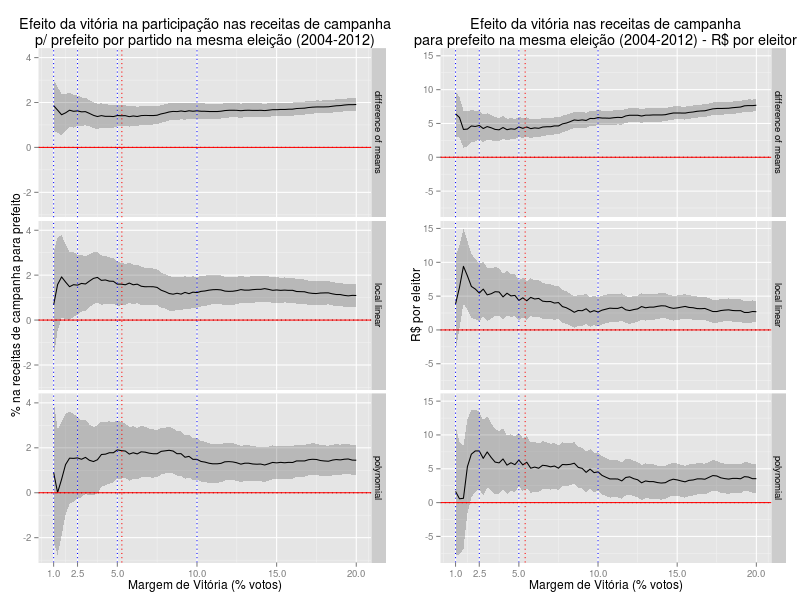
\includegraphics[scale=0.45]{c4pref1.png}
	\caption{Efeito do Tratamento nas receitas de campanha para vereador (R\$ por eleitor ou como razão do total que todos os partidos arrecadam) na mesma eleição e por margem de vitórias nas eleições para prefeito (2004-2008).}
	\label{fig:c4g1}
\end{figure}

Em ambos os casos vemos que há um claro desequilíbrio entre os grupos de tratamento, mesmo para margens de vitória menores ou iguais a valores no intervalo $1\% \leq \Delta \leq 2,5\%$. Adotando o ponto $\Delta \leq 2,5\%$, referência utilizada ao longo da tese, vemos que partidos arrecadaram em município em que venceram em média R\$ 1,55 por eleitor ou 5,5\% do total arrecadados por todos os partidos a mais do que em municípios em que perderam. O resultado é bastante resistente à redução da margem de vitória.

Um detalhe importante a se observar é que assumo que a variável é de fato anterior -- ou pelo menos contemporânea -- à atribuição do tratamento. Esta característica da variável, porém, pode ser questionada. A prestação de contas de campanha publicada pelo TSE e utilizada na construção da tese ocorre apenas após o resultado das eleições. Se, por exemplo, candidatos vencedores tiverem sistematicamente mais incentivos para declarar todas as receitas de campanha (por exemplo, sob o risco de perderem o mandato se não o fizerem) do que os candidatos perdedores, então o desequilíbrio encontrado pode ser consequência de um problema de medição e não necessariamente de uma desigualdade entre vencedores e perdedores. Neste caso, a variável seria posterior à atribuição do tratamento e possivelmente consequência do resultado das eleições.

Vamos ignorar esta possibilidade e prosseguir assumindo que a variável está corretamente medida. O desequilíbrio nesta variável afeta todos os resultados da tese. Sistematicamente, partidos vencedores arrecadaram mais na eleição que determinou tratados e não tratados do que partidos perdedores. Como, então, contornar este problema?

\section{Controlando por observáveis em um desenho de regressão descontínua}

Umas das opções seria rever os resultados e considerar apenas efeitos do tratamento obtidos para margens de vitória realmente pequenas, por exemplo, que atendam à $\Delta \leq 1\%$. porém, sabemos que, salvo raras excessões, nenhum dos resultados da tese é diferente de zero para margens de vitória tão próximas a zero. Poucas eleiçõe atendem à condição $0\% \leq \Delta \leq 1\%$ para este invervalo a ausência de efeito se confunde com ausência de significância provocada pelo número baixo de observações.

A alternativa encontrada neste capítulo adicional é manter repetir a análise para margens de vitórias $\Delta \leq 2,5\%$ adotando as receitas de campanha dos candidatos como controle. Durante toda a tese assumi que era preciso comparar observações de partidos quase perdedores com quase ganhadores por considerar que todos os fatores que explicariam simultaneamente as variáveis dependentes ($Y_{i}$) e a probabilidade de tratamento era não observáveis. Provavelmente a maioria dos fatores presentes em $A_{i}$ de fato continuam desconhecidos ou são difíceis de serem medidos. A receita de campanha dos candidatos $a_{i}$ é um um dos fatores presentes em $A_{i}$. Em vez de viés em não observáveis, passamos para uma situação de viés em observáveis. Uma vez que $a_{i}$ provoca desigualdades entre os grupos de tratamento, é possível rever os resultados controlando por $a_{i}$.

Sob este novo problema, podemos reescrever a probabilidade de tratamento como sendo: 

\[
\lim_{\Delta \to 0} E[d_{i}|\tau_{i}=-\Delta,a_{i}]=\lim_{\Delta \to 0} E[d_{i}|\tau_{i}=+\Delta,a_{i}]
\]

O efeito causal $\rho$ pode ser reescrito como: 

\[\rho =\lim_{\Delta \to 0} E[E[Y_{i}|d_{i}=1]|\tau_{i}=+\Delta,a_{i}] - \lim_{\Delta \to 0} E[E[Y_{i}|d_{i}=0]|\tau_{i}=-\Delta,a_{i}]\]
\[=\lim_{\Delta \to 0} E[Y_{1,i}|\tau_{i}=+\Delta,a_{i}] - \lim_{\Delta \to 0} E[Y_{0,i}|\tau_{i}=-\Delta,a_{i}]\]
\[=\lim_{\Delta \to 0} (E[Y_{1,i}|\tau_{i}=+\Delta,a_{i}] - E[Y_{0,i}|\tau_{i}=-\Delta,a_{i}])\] 

E a estimativa de $\rho$ como descontinuidade em uma função linear obtida por:

\[Y_{i}=\beta_{0}+\rho*d_{i}+\beta_{1}*\tau_{i}+\beta_{a}*a_{i}+\epsilon_{i}\]


É fundamental notar que a receita de campanha para prefeito é uma das variáveis com menor disponibilidade no tempo. Os resultados revistos dos capítulos anteriores contém, na melhor das hipóteses, dados para os prefeitos eleitos em 2004 e 2008. Para as demais eleições só é possível tratar $a_{i}$ como não observável.

\section{Revendo os resultados dos capítulos anteriores controlando por viés em observáveis}

As Tabelas~\ref{tab:c4t1},~\ref{tab:c4t2},~\ref{tab:c4t4} e~\ref{tab:c4t5} apresentam as regressões para as observações que atendem à condição $\Delta \leq 2,5\%$ e repentem os principais resultados apresentados no Capítulo~\ref{cap:eleicoes}. As Tabelas~\ref{tab:c4t1} e~\ref{tab:c4t2} trazem o impacto estimado da vitória nas eleições municipais sobre o voto do partido para deputado federal e deputado estadual. Além dos resultados para todos as observações a partir de 2004, observo o esfeitos para o ano de 2008 em separado, por contexto eleitoral local (prefeitos incumbentes ou desafiantes), também apenas para 2008. A Tabela~\ref{tab:c4t1} traz os resultados para deputado federal e a Tabela~\ref{tab:c4t2} para deputado estadual. Em baixo de cada tabela há uma explicação curta de cada uma das especificações.

\input c4t1
\input c4t2
%\input c4t3

Os resutados para deputado federal apresentados nesta seção continuam bastante expressivos. O partido tende a ter um desempenho 3,45\% (Especificação 1 da Tabela~\ref{tab:c4t1}) nos municipios nos quais venceu as eleições para prefeito. Em municípios onde o partido não governava anteriormente (prefeito desafiante, apresentado na Especificação 4 da Tabela~\ref{tab:c4t1}), o impacto de vencer as eleições sobre a performance do partido sobe para 5,45\%.

O efeito do tratamento nos votos do partido para deputado estadual nas eleições seguintes é positivo e diferente de zero apenas quando circunscrevemos a análise aos municípios em que o partido era desafiante na disputa municipal (Especificação 4 da Tabela~\ref{tab:c4t2}). Nestas situações, vencer as eleições para prefeito melhora em 4,3\% a performance do partido no municipio na disputa pelo Legislativo estadual. Vale notar que em nenhum das especificações das duas tabelas o coeficiente das receitas de campanha para prefeiuto difere de zero.

De maneira bastante breve, podemos reassegurar os resultados encontrados no primeiro capítulo para o impacto do partido governar o município no desempenho do partido nas eleições proprorcionais estaduais e nacionais, sobretudo a partir de 2008. Vamos agora examinar se os resultados para os demais cargos são diferentes dos encontrados anteriormente.

\input c4t4
\input c4t5

A Tabela~\ref{tab:c4t4} traz os resultado para a disputa para o Senado Federal. As duas primeiras especificações apresentam os resultados para 2004 e 2008, em separado. As duas útlimas repetem o procedimento excluindo o partido DEM, que, como vimos anteriormente, tinha resultados muito diferente dos demais partidos. O que encontramos são resultados nulos em qualquer especificação e não devemos esperar efeito do partido governar o município nos desempenho de seus candidatos para o Senado. Este resultado pouco altera o que encontramos anteriormente.

Por sua vez a Tabela~\ref{tab:c4t5} apresenta os resultados revistos do efeito do vitória local nos votos do partido para governador e presidente, agora introduzindo as receitas de campanha do partido nas eleições municipais como controle. As três primeiros especificações estimam o efeito do tratamento para todas as observações válidas, para governadores incumbentes e para governadores desafiantes, respectivamente. As duas últimas especificações apresentam os resultados para a disputa presidencial, já separados respectivamente pelo dois únicos partidos que importam na análise deste problema, PT e PSDB. Não há nenhum efeito do partido governar o município nos votos do partido para governador. Porém, seguimos com um efeito negativo especificamente para o PT nas eleições presidenciais (Especificação 4 da Tabela~\ref{tab:c4t4}). Certamente, este ´e um resultado não esperado que merece investigação no futuro.

As Tabelas~\ref{tab:c4t6} e~\ref{tab:c4t7} refazem os resultados do Capítulo~\ref{cap:emendas} apresentando o efeito do partido governar o município nas decisões dos deputados federais ao apresentar emendas individuais que beneficiem prefeituras (Tabela~\ref{tab:c4t6}) ou o conjunto de ESLFs (Tabela~\ref{tab:c4t7}) em uma determinadas localidades. Cada especificação apresenta os resultados para uma das medidas da variável depedente, que representa o total em emendas individuais apresentadas pelos parlamentares de um partido para organizações locais (prefeituras ou ESFLs) por algum dos seguintes denominadores, nesta ordem: total de eleitores aptos; receitas totais da prefeitura; total em emendas individuais apresentas por todos os partidos para a localidade (para prefeituras ou ESFLs); e o total de emendas apresentadas pelos deputados federais do partido para qualquer município (também separado por beneficiário).

\input c4t6
\input c4t7

Os resultados do Capítulo~\ref{cap:emendas} praticamente se mantém. Mesmo controlando por potenciais vieses provocados pelas desigualdades entre tratados e não tratados quanto às receitas de campanha na disputa pelo Executivo municipal, ainda encontramos efeitos importantes do partido governar o município nas decisões orçamentárias dos parlamentares de sua bancada. Esperamos que os deputados federais de um partido destinem em média R\$ 21,5 a mais por eleitor para municípios governados por prefeitos aliados do que para as demais localidades (Especificação 1 da Tabela~\ref{tab:c4t6}) e aloquem em média 13\% a mais de suas emendas para tais municípios em comparação com os demais (Especificação 4 da Tabela~\ref{tab:c4t6}).

Também acompanhando os resultados anteriormente apresentados, a Tabela~\ref{tab:c4t7} reapresenta o efeito do tratamento na decisão dos parlamentares alocarem recursos para ESFL. O efeito não é diferente de zero para as poucas observações próximas ao ponto em que temos uma correta identificação do efeito causal.

Finalmente, as Tabelas~\ref{tab:c4t8} e~\ref{tab:c4t9} trazem os resultados revistos do Capítulo~\ref{cap:mecanismos} após a introdução das receitas de campanha na disputa para prefeito como controle. Os resultados encontrados naquele capítulo, já bastante frágeis e praticamente indiferenciáveis de zero continuam inalterados. A Tabela~\ref{tab:c4t8} apresenta a estimação do efeito causal quando a variável dependente é o número de filiados, por eleitor apto (Especificação 1) ou a variação ao longo do mandato do prefeito (Especificação 2), e repete os resultados para o número de filiados ao partido na metade do mandato (Especificação 3 e 4). Na Tabela~\ref{tab:c4t9} estão as regressões e os coeficientes estimados para as duas medidas de receitas de campanha para vereador (por eleitor ou como proporção do total arrecadado por todos os partidos) e para as duas medidas de tamanho da coligação eleitoral (em número de partidos ou participação dos partidos da coligação no Legislativo local). Os resultados, como esperado, são nulos para os três problemas investigados e qualquer umadas medidas.

\input c4t8
\input c4t9

\section{Breve discussão: revendo (e mantendo) os resultados dos capítulos anteriores ao controlar por observáveis}

O propósito deste capítulo foi introduzir na estimação dos efeitos causais uma variável de controle que, no processo de elaborção da pesquisa, apareceu como uma diferença sistemática entre partidos eleitos e não eleitos: as receitas de campanha dos candidatos a prefeito. Havendo desigualdades entre os grupos de tratamento, os resultados produzidos anteriormente poderiam conter viés e, eventualmente, as conclusões obtidas a partir deles estariam equivocadas.

Os resultados gerais revistos neste capítulo pouco alteram as conclusões dos demais. Continuamos observando efeitos importantes da vitória nas eleições municipais sobre os votos do partido nas eleições proporcionais e na decisão dos deputados federais do partido ao apresentar emendas ao orçamento. Da mesma maneira, os resultados anteriormente nulos ou instáveis permancem inalterados.

Tendo em vista que o desequilíbrio entre grupos de tratamento encontrado não afeta os resultados, podemos avançar para a discussão final da tese.